\section{Results: Reading Is Not Writing Across Models}
\label{sec:campaign}

\subsection{The seed findings replicate on new patients}
\label{sec:campaign-replication}

The campaign re-runs Qwen2.5-VL-7B on a 600-image NIH cohort disjoint from every earlier cohort, with the six-direction matrix, 119 random directions, and the sham at $\alpha=+0.25$. Effusion again satisfies the steering reference: $W_{\mathrm{Effusion},\mathrm{Effusion}}=0.190$, above the random 95th percentile of 0.137 and the absolute sham of 0.017, ranking second among the 120 compared effects. Nodule again realises the maximum competing effect, and the ownership contrast is $O_{\mathrm{Effusion}}=-0.071$ (95\% CI $[-0.080,-0.062]$), matching the original $-0.057$ $[-0.069,-0.045]$ in sign and magnitude. All six diagonal ownership contrasts are negative ($-0.07$ to $-0.23$), as in the original matrix. The Mass wording dependence reproduces as well: under the \emph{show} A/B templates the Mass ownership contrast is positive while under the \emph{is} templates it is negative (Appendix~\ref{app:cf-transfer}).

\subsection{Readable and answerable, rarely owned}
\label{sec:campaign-grid}

Table~\ref{tab:cf-leaderboard} grades every completed block, and Figure~\ref{fig:cf-read-write} places every checkpoint--concept cell on the readability--ownership plane.

\begin{table}[t]
\centering
\scriptsize
\setlength{\tabcolsep}{2pt}
\renewcommand{\arraystretch}{1.08}
% Morandi tints for the cf-transfer tables (muted, low saturation); darker = larger value
\definecolor{cfSage1}{HTML}{EEF1EA}
\definecolor{cfSage2}{HTML}{D9E1D2}
\definecolor{cfSage3}{HTML}{C1CDB8}
\definecolor{cfSage4}{HTML}{A6B79C}
\definecolor{cfSlate1}{HTML}{ECEFF2}
\definecolor{cfSlate2}{HTML}{D3DAE2}
\definecolor{cfSlate3}{HTML}{B7C3D0}
\definecolor{cfSlate4}{HTML}{98A8B9}
\definecolor{cfTerra1}{HTML}{F5ECE9}
\definecolor{cfTerra2}{HTML}{E9D3CC}
\definecolor{cfTerra3}{HTML}{DAB5AA}
\definecolor{cfTerra4}{HTML}{C9968A}
\definecolor{cfOat1}{HTML}{F4EFE6}
\definecolor{cfOat2}{HTML}{E8DDC8}
\definecolor{cfGrey}{HTML}{E4E1DC}

\caption{\textbf{Reading, answering, and writing per checkpoint.} Per dataset: mean probe selectivity (\textsc{Read}), clean-answer AUROC (\textsc{Ans}), and ownership (\textsc{Own}), superscripted with the graded concepts of six, then the owned share of clinical and COCO cells and their ratio. Grey marks an ineligible template (inel.), an incomplete write matrix (inc.); ``--'' is a block not run.}
\label{tab:cf-main}
\begin{tabular}{l@{\hspace{3pt}}ccc@{\hspace{4pt}}ccc@{\hspace{4pt}}ccc@{\hspace{4pt}}ccc}
\toprule
& \multicolumn{3}{c}{NIH ChestX-ray14} & \multicolumn{3}{c}{CheXpert Plus} & \multicolumn{3}{c}{COCO (control)} & \multicolumn{3}{c}{Owned share} \\
\cmidrule(lr){2-4}\cmidrule(lr){5-7}\cmidrule(lr){8-10}\cmidrule(lr){11-13}
Checkpoint & \textsc{Read} & \textsc{Ans} & \textsc{Own} & \textsc{Read} & \textsc{Ans} & \textsc{Own} & \textsc{Read} & \textsc{Ans} & \textsc{Own} & clin. & COCO & ratio \\
\midrule
Lingshu 32B & \cellcolor{cfSage2}0.08$^{3}$ & \cellcolor{cfSage3}0.78$^{6}$ & \cellcolor{cfTerra2}-0.02$^{2}$ & \cellcolor{cfSage4}0.20$^{4}$ & \cellcolor{cfSage3}0.87$^{5}$ & \cellcolor{cfSlate2}+0.04$^{5}$ & \cellcolor{cfSage1}0.03$^{1}$ & \cellcolor{cfSage4}0.95$^{5}$ & \cellcolor{cfSlate4}+0.28$^{6}$ & \cellcolor{cfSlate4}58\% & \cellcolor{cfSlate4}100\% & 58\% \\
CheXagent-2-3B & \cellcolor{cfSage3}0.13$^{5}$ & \cellcolor{cfSage3}0.86$^{6}$ & \cellcolor{cfSlate1}+0.00$^{2}$ & \cellcolor{cfSage4}0.21$^{5}$ & \cellcolor{cfSage4}0.95$^{5}$ & \cellcolor{cfSlate1}+0.01$^{4}$ & \cellcolor{cfSage3}0.13$^{4}$ & \cellcolor{cfSage3}0.81$^{5}$ & \cellcolor{cfSlate2}+0.03$^{2}$ & \cellcolor{cfSlate4}50\% & \cellcolor{cfSlate2}33\% & 150\% \\
Qwen2.5-VL-72B & \cellcolor{cfSage2}0.07$^{2}$ & \cellcolor{cfSage2}0.62$^{4}$ & \cellcolor{cfTerra2}-0.03$^{3}$ & \cellcolor{cfSage3}0.20$^{4}$ & \cellcolor{cfSage2}0.71$^{4}$ & \cellcolor{cfTerra2}-0.09$^{1}$ & \cellcolor{cfSage1}0.01$^{1}$ & \cellcolor{cfSage4}0.99$^{5}$ & \cellcolor{cfSlate4}+0.66$^{6}$ & \cellcolor{cfSlate3}33\% & \cellcolor{cfSlate4}100\% & 33\% \\
Lingshu 7B & \cellcolor{cfSage2}0.08$^{3}$ & \cellcolor{cfSage3}0.76$^{6}$ & \cellcolor{cfSlate2}+0.02$^{1}$ & \cellcolor{cfSage4}0.21$^{4}$ & \cellcolor{cfSage3}0.86$^{5}$ & \cellcolor{cfSlate2}+0.04$^{3}$ & \cellcolor{cfSage1}0.02$^{1}$ & \cellcolor{cfSage4}0.97$^{5}$ & \cellcolor{cfSlate4}+0.68$^{6}$ & \cellcolor{cfSlate3}33\% & \cellcolor{cfSlate4}100\% & 33\% \\
Qwen3-VL-4B & \cellcolor{cfSage2}0.08$^{3}$ & \cellcolor{cfSage2}0.71$^{6}$ & \cellcolor{cfTerra3}-0.11$^{0}$ & \cellcolor{cfSage4}0.20$^{4}$ & \cellcolor{cfSage2}0.74$^{4}$ & \cellcolor{cfTerra1}-0.01$^{2}$ & \cellcolor{cfSage1}0.04$^{4}$ & \cellcolor{cfSage4}0.99$^{5}$ & \cellcolor{cfSlate4}+0.34$^{6}$ & \cellcolor{cfSlate3}17\% & \cellcolor{cfSlate4}100\% & 17\% \\
Qwen3-VL-32B & \cellcolor{cfSage2}0.10$^{2}$ & \cellcolor{cfSage2}0.70$^{6}$ & \cellcolor{cfTerra2}-0.02$^{1}$ & \cellcolor{cfSage3}0.17$^{5}$ & \cellcolor{cfSage3}0.82$^{5}$ & \cellcolor{cfTerra2}-0.02$^{1}$ & \cellcolor{cfSage2}0.05$^{4}$ & \cellcolor{cfSage4}0.99$^{5}$ & \cellcolor{cfSlate3}+0.15$^{6}$ & \cellcolor{cfSlate3}17\% & \cellcolor{cfSlate4}100\% & 17\% \\
InternVL3.5-38B & \cellcolor{cfSage2}0.10$^{5}$ & \cellcolor{cfSage3}0.78$^{6}$ & \cellcolor{cfTerra1}-0.00$^{0}$ & \cellcolor{cfSage3}0.17$^{4}$ & \cellcolor{cfSage3}0.86$^{5}$ & \cellcolor{cfTerra1}-0.00$^{2}$ & \cellcolor{cfSage2}0.08$^{4}$ & \cellcolor{cfSage4}0.99$^{5}$ & \cellcolor{cfSlate1}+0.01$^{6}$ & \cellcolor{cfSlate3}17\% & \cellcolor{cfSlate4}100\% & 17\% \\
Gemma 3 12B & \cellcolor{cfSage2}0.07$^{2}$ & \cellcolor{cfSage2}0.62$^{5}$ & \cellcolor{cfTerra4}-0.37$^{1}$ & \cellcolor{cfSage3}0.18$^{4}$ & \cellcolor{cfSage1}0.52$^{0}$ & \cellcolor{cfTerra4}-0.38$^{1}$ & \cellcolor{cfSage2}0.07$^{5}$ & \cellcolor{cfSage4}0.95$^{5}$ & \cellcolor{cfSlate4}+0.44$^{6}$ & \cellcolor{cfSlate3}17\% & \cellcolor{cfSlate4}100\% & 17\% \\
MedGemma 4B & \cellcolor{cfSage3}0.12$^{3}$ & \cellcolor{cfSage3}0.80$^{6}$ & \cellcolor{cfTerra3}-0.13$^{0}$ & \cellcolor{cfSage4}0.21$^{4}$ & \cellcolor{cfSage3}0.87$^{5}$ & \cellcolor{cfTerra3}-0.16$^{2}$ & \cellcolor{cfSage2}0.06$^{4}$ & \cellcolor{cfSage4}0.94$^{5}$ & \cellcolor{cfSlate3}+0.23$^{6}$ & \cellcolor{cfSlate3}17\% & \cellcolor{cfSlate4}100\% & 17\% \\
InternVL3.5-14B & \cellcolor{cfSage2}0.07$^{4}$ & \cellcolor{cfSage2}0.73$^{6}$ & \cellcolor{cfTerra1}-0.00$^{1}$ & \cellcolor{cfSage3}0.16$^{4}$ & \cellcolor{cfSage3}0.87$^{5}$ & \cellcolor{cfSlate1}+0.00$^{1}$ & \cellcolor{cfSage3}0.12$^{4}$ & \cellcolor{cfSage4}0.98$^{5}$ & \cellcolor{cfSlate1}+0.02$^{5}$ & \cellcolor{cfSlate3}17\% & \cellcolor{cfSlate3}83\% & 20\% \\
Qwen2.5-VL-32B & \cellcolor{cfSage2}0.09$^{3}$ & \cellcolor{cfSage2}0.63$^{4}$ & \cellcolor{cfTerra2}-0.06$^{1}$ & \cellcolor{cfSage3}0.16$^{4}$ & \cellcolor{cfSage2}0.70$^{4}$ & \cellcolor{cfTerra3}-0.11$^{0}$ & \cellcolor{cfSage1}0.02$^{1}$ & \cellcolor{cfSage4}0.99$^{5}$ & \cellcolor{cfSlate4}+0.38$^{6}$ & \cellcolor{cfSlate2}8\% & \cellcolor{cfSlate4}100\% & 8\% \\
InternVL3.5-8B & \cellcolor{cfSage2}0.06$^{2}$ & \cellcolor{cfSage2}0.73$^{6}$ & \cellcolor{cfTerra1}-0.01$^{0}$ & \cellcolor{cfSage3}0.19$^{4}$ & \cellcolor{cfSage3}0.86$^{5}$ & \cellcolor{cfTerra1}-0.00$^{1}$ & \cellcolor{cfSage2}0.12$^{5}$ & \cellcolor{cfSage4}0.98$^{5}$ & \cellcolor{cfSlate2}+0.03$^{6}$ & \cellcolor{cfSlate2}8\% & \cellcolor{cfSlate4}100\% & 8\% \\
HuatuoGPT-Vision-7B & \cellcolor{cfSage2}0.08$^{3}$ & \cellcolor{cfSage2}0.71$^{6}$ & \cellcolor{cfTerra2}-0.03$^{1}$ & \cellcolor{cfSage3}0.19$^{4}$ & \cellcolor{cfSage3}0.78$^{4}$ & \cellcolor{cfTerra1}-0.01$^{0}$ & \cellcolor{cfSage2}0.07$^{4}$ & \cellcolor{cfSage4}0.99$^{5}$ & \cellcolor{cfSlate1}+0.01$^{4}$ & \cellcolor{cfSlate2}8\% & \cellcolor{cfSlate3}67\% & 12\% \\
LLaVA-Med 1.5 7B & \cellcolor{cfSage2}0.08$^{3}$ & \cellcolor{cfSage1}0.53$^{0}$ & \cellcolor{cfTerra1}-0.01$^{0}$ & \cellcolor{cfSage3}0.19$^{4}$ & \cellcolor{cfSage1}0.59$^{2}$ & \cellcolor{cfTerra1}-0.01$^{1}$ & \cellcolor{cfSage2}0.07$^{4}$ & \cellcolor{cfSage3}0.76$^{5}$ & \cellcolor{cfSlate1}+0.00$^{1}$ & \cellcolor{cfSlate2}8\% & \cellcolor{cfSlate2}17\% & 50\% \\
CheXagent-8B & \cellcolor{cfSage3}0.16$^{5}$ & \cellcolor{cfSage2}0.73$^{6}$ & \cellcolor{cfTerra1}-0.00$^{0}$ & \cellcolor{cfSage4}0.23$^{5}$ & \cellcolor{cfSage3}0.88$^{5}$ & \cellcolor{cfTerra1}-0.02$^{1}$ & \cellcolor{cfSage2}0.05$^{3}$ & \cellcolor{cfSage1}0.52$^{1}$ & \cellcolor{cfTerra2}-0.03$^{0}$ & \cellcolor{cfSlate2}8\% & \cellcolor{cfSlate1}0\% & -- \\
Qwen2.5-VL-3B & \cellcolor{cfSage2}0.07$^{2}$ & \cellcolor{cfSage1}0.58$^{2}$ & \cellcolor{cfTerra2}-0.08$^{0}$ & \cellcolor{cfSage3}0.17$^{4}$ & \cellcolor{cfSage1}0.57$^{2}$ & \cellcolor{cfTerra2}-0.07$^{0}$ & \cellcolor{cfSage1}0.05$^{4}$ & \cellcolor{cfSage4}0.97$^{5}$ & \cellcolor{cfSlate4}+0.52$^{6}$ & \cellcolor{cfSlate1}0\% & \cellcolor{cfSlate4}100\% & 0\% \\
Qwen2.5-VL-7B & \cellcolor{cfSage2}0.08$^{3}$ & \cellcolor{cfSage2}0.62$^{3}$ & \cellcolor{cfTerra3}-0.14$^{0}$ & \cellcolor{cfSage3}0.20$^{4}$ & \cellcolor{cfSage2}0.65$^{2}$ & \cellcolor{cfTerra2}-0.08$^{0}$ & \cellcolor{cfSage1}0.02$^{1}$ & \cellcolor{cfSage4}0.98$^{5}$ & \cellcolor{cfSlate4}+0.67$^{6}$ & \cellcolor{cfSlate1}0\% & \cellcolor{cfSlate4}100\% & 0\% \\
Qwen3-VL-8B & \cellcolor{cfSage2}0.10$^{4}$ & \cellcolor{cfSage2}0.69$^{6}$ & \cellcolor{cfTerra1}-0.01$^{0}$ & \cellcolor{cfSage3}0.17$^{4}$ & \cellcolor{cfSage2}0.75$^{4}$ & \cellcolor{cfTerra2}-0.04$^{0}$ & \cellcolor{cfSage1}0.04$^{3}$ & \cellcolor{cfSage4}0.99$^{5}$ & \cellcolor{cfSlate4}+0.58$^{6}$ & \cellcolor{cfSlate1}0\% & \cellcolor{cfSlate4}100\% & 0\% \\
Gemma 3 27B & \cellcolor{cfSage2}0.07$^{2}$ & \cellcolor{cfSage2}0.60$^{3}$ & \cellcolor{cfTerra2}-0.03$^{0}$ & \cellcolor{cfSage3}0.18$^{4}$ & \cellcolor{cfSage1}0.55$^{2}$ & \cellcolor{cfTerra1}-0.01$^{0}$ & \cellcolor{cfSage2}0.07$^{5}$ & \cellcolor{cfSage4}0.96$^{5}$ & \cellcolor{cfSlate4}+0.31$^{6}$ & \cellcolor{cfSlate1}0\% & \cellcolor{cfSlate4}100\% & 0\% \\
Gemma 3 4B & \cellcolor{cfSage2}0.07$^{2}$ & \cellcolor{cfSage1}0.56$^{2}$ & \cellcolor{cfTerra3}-0.11$^{0}$ & \cellcolor{cfSage3}0.18$^{4}$ & \cellcolor{cfSage1}0.53$^{1}$ & \cellcolor{cfTerra4}-0.27$^{0}$ & \cellcolor{cfSage2}0.07$^{5}$ & \cellcolor{cfSage4}0.94$^{5}$ & \cellcolor{cfSlate3}+0.24$^{5}$ & \cellcolor{cfSlate1}0\% & \cellcolor{cfSlate3}83\% & 0\% \\
LLaVA-1.5-7B & \cellcolor{cfSage2}0.08$^{2}$ & \cellcolor{cfSage1}0.51$^{0}$ & \cellcolor{cfTerra2}-0.04$^{0}$ & \cellcolor{cfSage3}0.17$^{4}$ & \cellcolor{cfSage1}0.52$^{0}$ & \cellcolor{cfTerra2}-0.03$^{0}$ & \cellcolor{cfSage4}0.28$^{5}$ & \cellcolor{cfSage4}0.97$^{5}$ & \cellcolor{cfSlate2}+0.03$^{5}$ & \cellcolor{cfSlate1}0\% & \cellcolor{cfSlate3}83\% & 0\% \\
MedGemma 27B & \cellcolor{cfSage3}0.12$^{3}$ & \cellcolor{cfSage3}0.80$^{6}$ & \cellcolor{cfTerra3}-0.14$^{0}$ & \cellcolor{cfSage4}0.21$^{4}$ & \cellcolor{cfSage3}0.87$^{5}$ & \cellcolor{cfTerra2}-0.06$^{0}$ & \cellcolor{cfSage2}0.06$^{4}$ & \cellcolor{cfSage4}0.97$^{5}$ & \cellcolor{cfSlate3}+0.12$^{4}$ & \cellcolor{cfSlate1}0\% & \cellcolor{cfSlate3}67\% & 0\% \\
LLaVA-1.5-13B & \cellcolor{cfSage2}0.08$^{2}$ & \cellcolor{cfSage1}0.53$^{0}$ & \cellcolor{cfTerra2}-0.02$^{0}$ & \cellcolor{cfSage3}0.17$^{4}$ & \cellcolor{cfSage1}0.51$^{1}$ & \cellcolor{cfTerra1}-0.01$^{0}$ & \cellcolor{cfSage4}0.28$^{5}$ & \cellcolor{cfSage4}0.96$^{5}$ & \cellcolor{cfSlate2}+0.02$^{2}$ & \cellcolor{cfSlate1}0\% & \cellcolor{cfSlate2}33\% & 0\% \\
Llama 3.2 Vision 11B & \cellcolor{cfSage2}0.08$^{2}$ & \cellcolor{cfSage2}0.65$^{4}$ & \cellcolor{cfTerra2}-0.03$^{0}$ & \cellcolor{cfSage3}0.16$^{4}$ & \cellcolor{cfSage2}0.73$^{4}$ & \cellcolor{cfTerra2}-0.04$^{0}$ & \cellcolor{cfSage3}0.12$^{5}$ & \cellcolor{cfSage4}0.95$^{5}$ & \cellcolor{cfTerra1}-0.01$^{1}$ & \cellcolor{cfSlate1}0\% & \cellcolor{cfSlate2}17\% & 0\% \\
LLaVA-Rad-7B & \cellcolor{cfSage3}0.15$^{4}$ & \cellcolor{cfSage2}0.71$^{5}$ & \cellcolor{cfTerra1}-0.01$^{0}$ & \cellcolor{cfSage4}0.27$^{5}$ & \cellcolor{cfSage3}0.87$^{5}$ & \cellcolor{cfTerra1}-0.02$^{0}$ & \cellcolor{cfSage3}0.12$^{4}$ & \cellcolor{cfSage1}0.50$^{0}$ & \cellcolor{cfTerra2}-0.03$^{0}$ & \cellcolor{cfSlate1}0\% & \cellcolor{cfSlate1}0\% & -- \\
\midrule
\textbf{All cells} & 0.09 & 0.68 & -0.06 & 0.19 & 0.74 & -0.05 & 0.08 & 0.92 & +0.23 & 13\% & 75\% & 17\% \\
\quad count / cells & 74/150 & 110/150 & 13/150 & 104/150 & 89/150 & 25/150 & 90/150 & 116/150 & 113/150 & & & \\
\bottomrule
\end{tabular}
\end{table}



\begin{figure}[t]
    \centering
    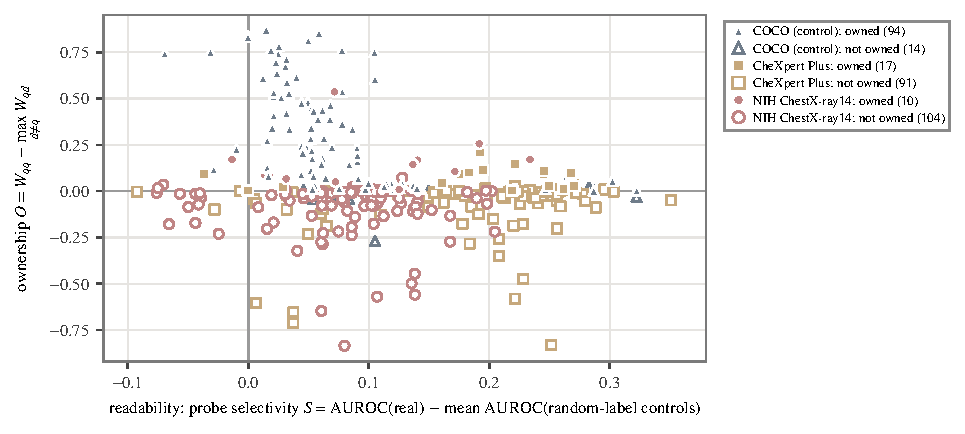
\includegraphics[width=0.72\textwidth]{figures/cf_F2_read_vs_write.pdf}
    \caption{\textbf{Every concept cell of the campaign.} Readability (probe selectivity $S$) against ownership ($O_q$) for all checkpoint--concept cells; filled markers are owned cells. Clinical cells (NIH, CheXpert) are readable across the whole range of $S$ and sit at or below zero ownership; COCO cells occupy the upper half.}
    \label{fig:cf-read-write}
\end{figure}

On NIH, 50 of 114 cells are readable, 77 are answerable, and 35 are both; 10 are owned. On CheXpert, 69 of 102 cells are readable, 55 answerable, 49 both, and 17 owned. In 78 NIH and 67 CheXpert cells the verdict is \emph{stronger competitor}: another clinical direction moves the concept's answer more than the concept's own direction, with a simultaneous upper bound below zero. Readability does not predict ownership: among the 84 clinical cells that are both readable and answerable, 19 are owned. The seed concept, Effusion, is owned in 5 of 36 chest blocks, four of them with $O_{\mathrm{Effusion}}\leq 0.03$, and is anti-owned by every Qwen2.5-VL size on NIH (Figure~\ref{fig:cf-effusion}).

\begin{figure}[t]
    \centering
    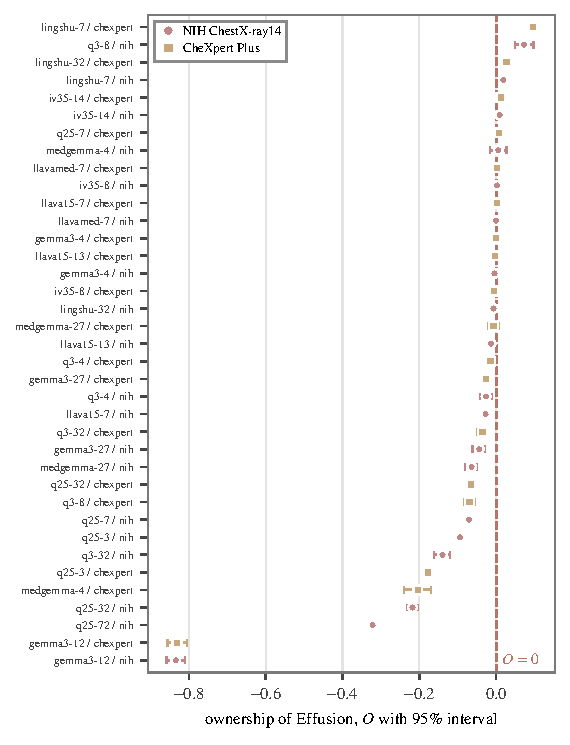
\includegraphics[width=0.58\textwidth]{figures/cf_F3_effusion_across_blocks.pdf}
    \caption{\textbf{Effusion in every chest block.} Ownership $O_{\mathrm{Effusion}}$ with 95\% percentile intervals for all 36 checkpoint--dataset blocks on NIH and CheXpert, sorted by estimate.}
    \label{fig:cf-effusion}
\end{figure}

Ownership, when it occurs, is concentrated in a few checkpoints and does not transfer across datasets: Qwen2.5-VL-72B owns Atelectasis ($O=0.54$), Cardiomegaly, and Mass on NIH; Lingshu-32B owns Pneumothorax and Cardiomegaly on NIH and five concepts on CheXpert; Qwen2.5-VL-32B owns Cardiomegaly on NIH but no CheXpert concept, where the same direction is anti-owned ($O=-0.19$). Different checkpoints own different single concepts (Table~\ref{tab:cf-leaderboard}).

\subsection{The write mechanism is intact: natural objects}
\label{sec:coco}

The same cohorts, directions, gates, and rules applied to COCO give the opposite picture (Table~\ref{tab:cf-leaderboard}, Figure~\ref{fig:cf-dose}). 94 of 108 cells are owned, with ownership contrasts of $0.1$--$0.9$ for the Qwen, Lingshu, and Gemma families; 96 cells meet the steering reference and only 6 receive the stronger-competitor verdict. Fourteen of fifteen checkpoints with a COCO block own all or most of the six objects; the exception, LLaVA-Med, reads them (selectivity $0.10$--$0.15$) and answers them but writes only one. Dose response is monotone on COCO and flat or negative on the chest sets: the median ownership across the six questions rises from $0$ at $\alpha=0$ to $0.4$--$0.9$ at $\alpha=0.5$ on COCO, while on NIH it stays within $\pm0.1$ for most checkpoints and falls for the rest.

\begin{figure}[t]
    \centering
    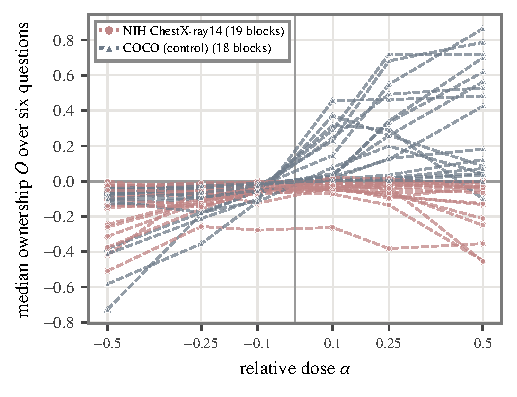
\includegraphics[width=0.62\textwidth]{figures/cf_F6_dose_response.pdf}
    \caption{\textbf{Dose response.} Median ownership over the six questions as a function of the relative dose $\alpha$ (DOSE module plus the $\alpha=+0.25$ CORE point), one line per block. COCO blocks rise monotonically; NIH blocks stay near zero or fall.}
    \label{fig:cf-dose}
\end{figure}

\subsection{Same write, different reader}
\label{sec:same-write}

Gemma~3 ships one SigLIP vision tower for its 4B, 12B, and 27B checkpoints, and MedGemma one MedSigLIP tower for 4B and 27B. Because the primary locus is the tower's final block, the pooled features, the fitted probes, and the write vectors are byte-identical across sizes within each family (verified by file hash for Gemma~3 4B/12B; equal up to bf16 rounding for 27B and for MedGemma, with direction cosines above 0.9987). What differs is the connector and language model that read the written representation. Figure~\ref{fig:cf-same-write} shows the outcome: with the same write, Gemma~3 4B owns nothing on either chest set, 12B owns Nodule on NIH and Edema on CheXpert, and 27B owns nothing; on COCO the three sizes own 5, 6, and 6 objects. MedGemma 4B owns Cardiomegaly and Edema on CheXpert and 27B owns neither. Readability is by construction identical across sizes, so every difference in these panels is a difference in writability alone.

\begin{figure}[t]
    \centering
    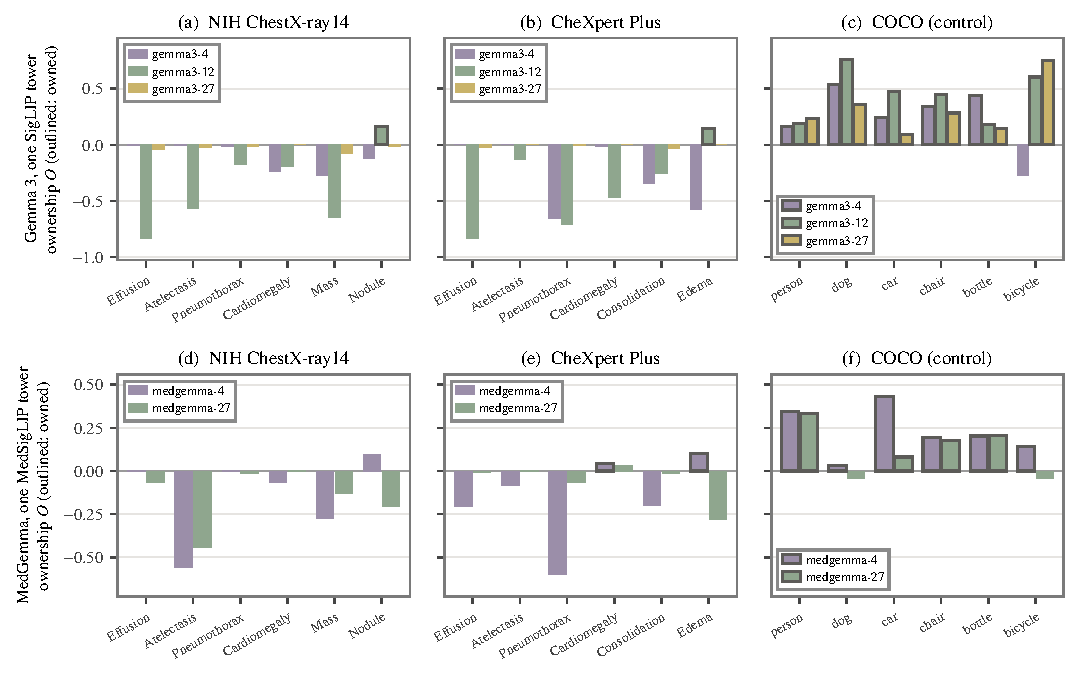
\includegraphics[width=\textwidth]{figures/cf_F4_same_write_different_reader.pdf}
    \caption{\textbf{Same write vector, different reader.} Ownership per concept for Gemma~3 4B/12B/27B (top) and MedGemma 4B/27B (bottom) on NIH, CheXpert, and COCO. Within a family the probes and write vectors are identical across sizes; outlined bars are owned.}
    \label{fig:cf-same-write}
\end{figure}

\subsection{Size ladders and families}
\label{sec:ladders}

Figure~\ref{fig:cf-ladders} follows four families across sizes on the chest sets. Qwen2.5-VL owns nothing at 3B and 7B, Cardiomegaly at 32B, and Atelectasis, Cardiomegaly, and Mass at 72B, while Effusion is anti-owned at every size. Qwen3-VL owns nothing at 4B and 8B and Nodule at 32B on NIH; on CheXpert it owns Consolidation and Edema at 4B and Edema at 32B. InternVL3.5 answers all six NIH questions at 8B and 14B, but its writes stay within $0.04$ of zero at both loci on every dataset except COCO, where it owns all six objects with small effects. Lingshu, the medical Qwen2.5-VL derivative, owns Cardiomegaly on NIH at 7B and adds Pneumothorax at 32B, and owns three CheXpert concepts at 7B and five at 32B. LLaVA-1.5 7B/13B and LLaVA-Med read chest concepts, answer none above chance, and own none; the 11B Llama~3.2~Vision fails the yes/no mapping gate on all datasets and is graded on its B-mapped templates only.

\begin{figure}[t]
    \centering
    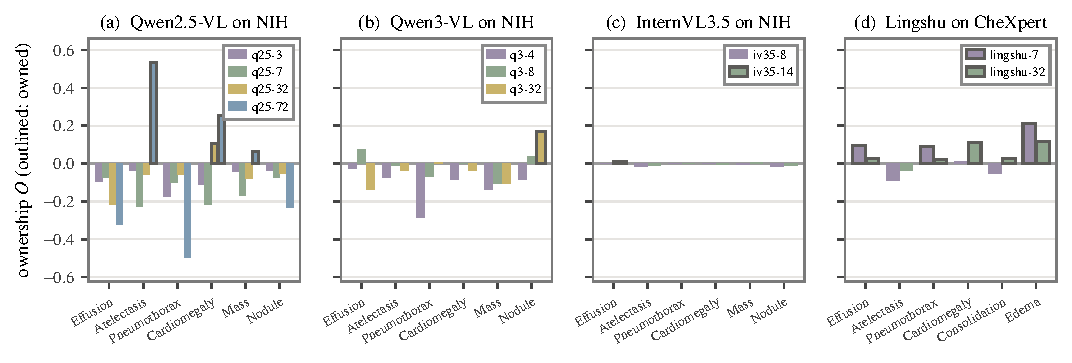
\includegraphics[width=\textwidth]{figures/cf_F7_size_ladders.pdf}
    \caption{\textbf{Size ladders.} Ownership per concept across sizes for Qwen2.5-VL and Qwen3-VL on NIH, InternVL3.5 on NIH, and Lingshu on CheXpert; outlined bars are owned.}
    \label{fig:cf-ladders}
\end{figure}

\subsection{Controls}
\label{sec:controls}

Every block carries the same controls (Figure~\ref{fig:cf-controls}). The reference family behaves as designed: owned cells sit beyond the 119 random writes and the sham, and the sham never exceeds an owned concept write (Figure~\ref{fig:cf-reference}). Writes at the connector locus are inert in every family: the connector-locus median ownership is within $\pm0.03$ of zero for all blocks except Gemma~3 12B on NIH ($-0.07$), while the primary-locus write moves answers by up to $0.9$. Refits over three seeds change ownership by a median of $0.02$--$0.06$ per block (up to $0.18$ for the Gemma family). Relabelling shifts the answer far more than the concept write on COCO (label-shift gaps of $-3$ to $-18$) and by less than $1$ on most chest blocks. The wording and mapping contrasts between templates are small for most families and large for Mass in Qwen2.5-VL and for bottle in Gemma~3 4B, reproducing the prompt dependence of Section~\ref{sec:encoding-results} (Appendix~\ref{app:cf-transfer}).

\begin{figure}[t]
    \centering
    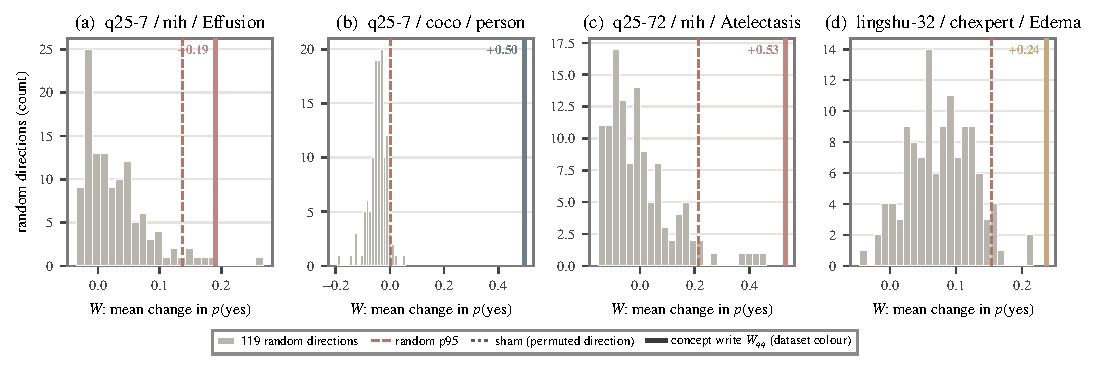
\includegraphics[width=0.9\textwidth]{figures/cf_F5_reference_family.pdf}
    \caption{\textbf{The steering reference.} The 119 random-direction writes (histogram), the coordinate-permutation sham, and the concept write for four blocks: Qwen2.5-VL-7B Effusion on NIH (reference met, ownership negative), Qwen2.5-VL-7B person on COCO, Qwen2.5-VL-72B Atelectasis on NIH, and Lingshu-32B Edema on CheXpert (all owned).}
    \label{fig:cf-reference}
\end{figure}

\begin{figure}[t]
    \centering
    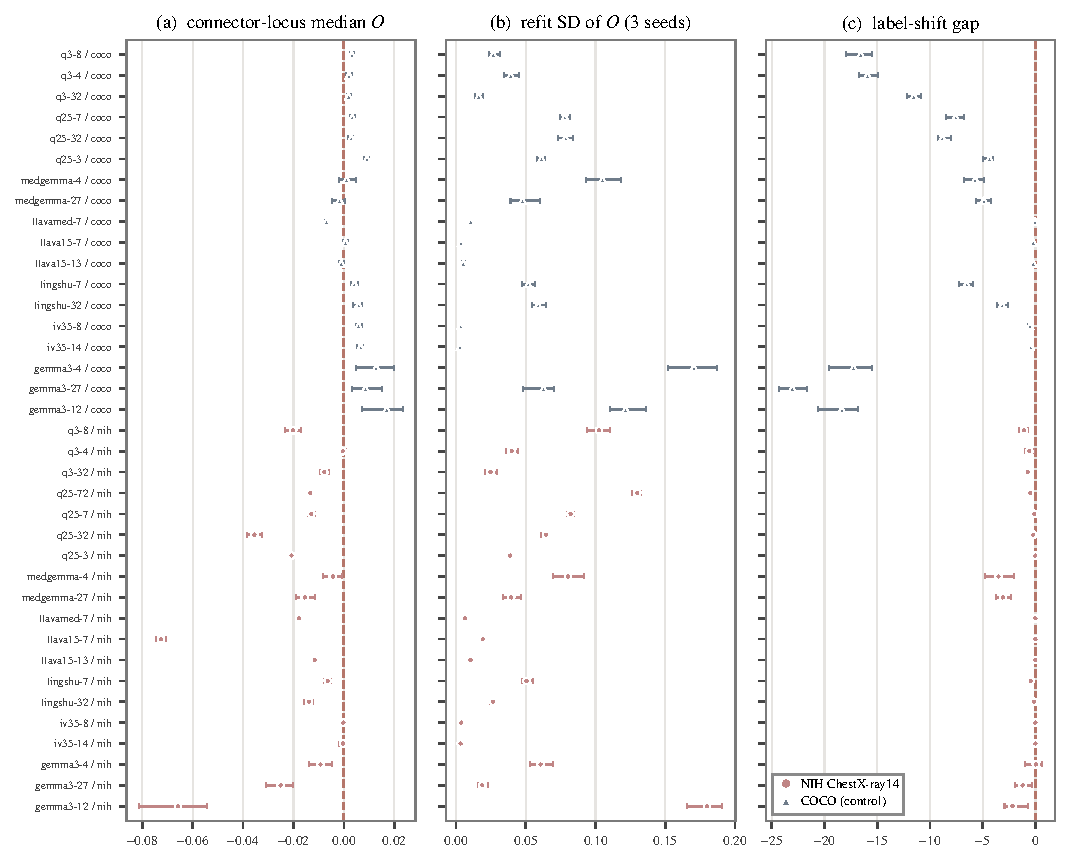
\includegraphics[width=\textwidth]{figures/cf_F9_controls.pdf}
    \caption{\textbf{Controls per block.} Connector-locus median ownership, refit standard deviation over three seeds, and label-shift gap for every block with the full module set.}
    \label{fig:cf-controls}
\end{figure}

\FloatBarrier
